\section*{Dynamical System}

A system of equations:
\begin{align*}
    \frac{dx}{dt} &= P(x, y) \\
    \frac{dy}{dt} &= Q(x, y)
\end{align*}
which represents a physical problem is called a \textbf{dynamical system}.

\subsubsection*{Example:}
Consider the system of equations:
\begin{align*}
    \frac{dx}{dt} &= x - y \\
    \frac{dy}{dt} &= -x + y
\end{align*}
This is a dynamical system.
\section*{Autonomous and Non-Autonomous Dynamical Systems}

An \textbf{autonomous dynamical system} is a system of differential equations in which the independent variable time $t$ does not explicitly appear in the defining functions.

\subsection*{Formulation}
In a two-dimensional system, it is represented as:
\begin{align*}
    \dot{x} &= \frac{dx}{dt} = P(x, y) \\
    \dot{y} &= \frac{dy}{dt} = Q(x, y)
\end{align*}
where the functions $P$ and $Q$ depend solely on the state variables $x$ and $y$, and not directly on $t$.

\subsection*{Non-Autonomous Dynamical System}
If the independent variable $t$ appears explicitly in the governing equations, the system is called a \textbf{non-autonomous system}:
\begin{align*}
    \dot{x} &= \frac{dx}{dt} = P(x, y, t) \\
    \dot{y} &= \frac{dy}{dt} = Q(x, y, t)
\end{align*}

\subsection*{Examples}

\subsubsection*{1. Autonomous System:}
\begin{align*}
    \dot{x} &= xy \\
    \dot{y} &= x^2 + y^2
\end{align*}
\noindent \textit{(No explicit time parameter $t$ on the right-hand side.)}

\subsubsection*{2. Non-Autonomous System:}
\begin{align*}
    \dot{x} &= xt + y \\
    \dot{y} &= x^2 + y^2 + t^2
\end{align*}
\noindent \textit{(Time parameter $t$ explicitly appears on the right-hand side.)}
\section*{Critical Point}

Let
\begin{equation}
    \dot{x} = P(x, y), \quad \dot{y} = Q(x, y) \sidenote{1}
\end{equation}
be a dynamical system. A point $(x_0, y_0)$ is called a \textbf{critical point} of the system (1) if:

\begin{enumerate}
    \item[(i)] $P(x_0, y_0) = 0$ \quad \text{and} \quad $Q(x_0, y_0) = 0$
\end{enumerate}

\noindent i.e.,
\begin{align*}
    \dot{x} &= 0 \\
    \dot{y} &= 0
\end{align*}

\section*{Isolated Critical Points}

Let
\begin{equation}
    \dot{x} = P(x, y) \quad \text{and} \quad \dot{y} = Q(x, y) \sidenote{i}
\end{equation}
be a dynamical system, and let $(x_0, y_0)$ be a critical point of (i). If there exists a neighborhood of the critical point $(x_0, y_0)$ such that no other critical point lies in that neighborhood, then $(x_0, y_0)$ is called an \textbf{isolated critical point}.

\vspace{0.5em}
\noindent There are four types of isolated critical points:
\begin{enumerate}
    \item[(i)] Node
    \item[(ii)] Saddle point
    \item[(iii)] Spiral (Focus)
    \item[(iv)] Center
\end{enumerate}
\section*{Node:}
Consider the autonomous dynamical system:
\[
\dot{x} = P(x, y), \quad \dot{y} = Q(x, y)
\]
with an isolated critical point at the origin $(0, 0)$. The critical point $(0, 0)$ is called a \textbf{node} if:

\begin{enumerate}
    \item Every trajectory in a neighborhood of $(0, 0)$ approaches $(0, 0)$ either as $t \to +\infty$ (stable node) or as $t \to -\infty$ (unstable node).
    \item Every trajectory enters or leaves $(0, 0)$ along a \textbf{well-defined tangent line} (a definite direction).
    \item Trajectories \textbf{do not spiral or rotate} infinitely around $(0, 0)$ as they approach or leave it.
\end{enumerate}

\subsection*{Alternative (Eigenvalue Criterion for Linear Systems)}

If the condition is given in terms of linear system dynamics ($\dot{\mathbf{x}} = A\mathbf{x}$):

\begin{quote}
\textit{The isolated critical point $(0, 0)$ is a \textbf{node} if the eigenvalues $\lambda_1, \lambda_2$ of the Jacobian matrix evaluated at $(0, 0)$ are \textbf{real, non-zero, distinct (or proper)}, and have the same sign:}
\begin{itemize}
    \item \textbf{Stable Node:} $\lambda_1, \lambda_2 < 0$ \textit{(Real and both negative)}
    \item \textbf{Unstable Node:} $\lambda_1, \lambda_2 > 0$ \textit{(Real and both positive)}
\end{itemize}
\end{quote}
\begin{center}
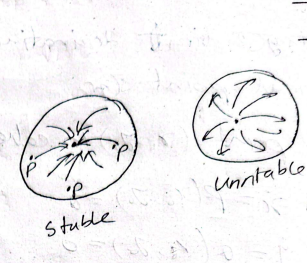
\includegraphics[width=0.6\textwidth]{Image/node.png}
\end{center}
